\documentclass[11pt]{article}
\renewcommand{\baselinestretch}{1.20} 
\usepackage[utf8]{inputenc}
\usepackage[english]{babel}
\usepackage{graphicx}
\usepackage{wrapfig}
\usepackage{subcaption}
\usepackage{geometry}
\usepackage{xcolor}
\usepackage{mdframed}
\usepackage{booktabs}% http://ctan.org/pkg/booktabs
\newcommand{\tabitem}{~~\llap{\textbullet}~~}
\geometry{a4paper, total={170mm,237mm}, left=20mm, top=30mm}
\setlength{\abovecaptionskip}{15pt plus 3pt minus 2pt}

\begin{document}
    
    %Title page
    \begin{titlepage}
    \centering
	
\includegraphics[width=0.35\textwidth]{Projectdoc/Assets/Illustrationer/aau_logo_en.pdf}\par\vspace{1cm}
	{\scshape\Large Interaction Design\par}
	\vspace{0.2cm}
	{\huge\bfseries Messages Hidden in Public\par}
	\vspace{0.2cm}
	{\scshape\Large ITC - B125\par}
	\vspace{2cm}
	{\Large\itshape 
    	Mikkel Steen Hansen\\
        Benjamin Bach Jensen\\
        Daniel Vestergaard Jensen\\
    \par}
	\vfill
	\vfill
\end{titlepage}
    
    % Table of contents
    \renewcommand{\baselinestretch}{0.8} 
    \tableofcontents
    \renewcommand{\baselinestretch}{1.20} 
    \newpage
    
    % Short project description
    \section{Short project description}
The goal of the project is to provide people with a tool to maintain some degree of freedom of speech, as well as independent thought, in dictatorial regimes. 
The goal has been chosen due to the potential future risks of ever increasing levels of monitoring across the globe. The intended users are therefore any citizen wanting to discuss the current state of affairs as well as activists that actively try to spread awareness in suppressed populations. The project could also be used by journalists working in the same regions. The military, or indeed intelligence services, might also be able to draw use from the same project. Although the potential benefits are numerous it is important to mention that secure communication could just as well be use by criminals to work against the needs of society.
    
    % Questionnaire description
    \section{Questionnaire methods and execution}
\noindent
This survey [View in appendix \ref{appendix:survey}] intends to explore the level of user awareness regarding privacy. \\
Firstly, it will be determined to which extent the individual user utilizes the internet.\\ 
Secondly, the type of user is determined. \\
Thirdly, the user is asked about their view on their personal privacy on the internet.\\
This is done to explore the possible correlation between amount of use, type of use and privacy view. \\
This information is intended to shed light on whether or not different user groups are likely to use a product capable of enhancing the security of their personal information and freedom on the internet.\\\\
\noindent
The questions in the survey were done in such a way as to allow for classification of the participants.
The survey also asked for permission to conduct follow-up interviews. These interviews intended to provide deeper insight into the reasoning behind certain behaviors. The individuals interviewed would bear close resemblance to one of the personas created to further enhance the insight into these personas.\\\\
\noindent
The intent of the survey was to clarify the archetypes of possible users to allow for the creation of a number of personas. These personas would then be used to create the relevant requirements for the product.
\noindent
Given that the participants have all been present at the university, studying some form of engineering, one possible error is that these participants might have a higher than average technical skill level as well as higher awareness of internet privacy issues.
    
    % Questionnaire survey
    %backgroundcolor=lightgray!20
\begin{mdframed}[linewidth=0pt,backgroundcolor=lightgray!20,innertopmargin = 0.1cm,innerbottommargin = 0.5cm]
    \noindent
    \textit{I hereby accept that my answers in this survey can be used in this study, on the condition that my anonymity is guaranteed.}\\
    \begin{tabular}{ll}
        Signature:\qquad
        \begin{left}
            \rule{0.6\textwidth}{.4pt}
        \end{left}
    \end{tabular}
    \begin{enumerate}
        \item What is your age ? \rule{0.1\textwidth}{.4pt}
        \item What are you currently studying ?
        \begin{left}
            \rule{0.46\textwidth}{.4pt}
        \end{left}
        
        \item ~For how long do you use your devices at home on average per day ? (Select \textbf{1})\\
        \begin{tabular}{ll}
            \tabitem Less than 2 hours & [\quad] \\
            \tabitem Around 2 to 4 hours & [\quad] \\
            \tabitem Around 4 to 6 hours & [\quad] \\
       
            \tabitem Around 6 to 8 hours & [\quad] \\
            \tabitem Around 8 to 10 hours & [\quad] \\
            \tabitem More than 10 hours & [\quad] \\
        \end{tabular}
        
        \item ~What do you primarily use your devices for ? (Select \textbf{at most 3}) \\
            \begin{minipage}{.5\textwidth}
                \begin{tabular}{ll}
                    \tabitem Homebanking & [\quad] \\
                    \tabitem Work & [\quad] \\
                    \tabitem School & [\quad] \\
                    \tabitem Entertainment (Youtube etc.) & [\quad] \\
                \end{tabular}
            \end{minipage}
            \begin{minipage}{.5\textwidth}
                \begin{tabular}{ll}
                    \tabitem Gaming & [\quad] \\
                    \tabitem Social networking & [\quad] \\
                    \tabitem Shopping & [\quad] \\
                    \tabitem Hobby & [\quad] \\
                \end{tabular}
            \end{minipage}
            \\\\
            \begin{tabular}{ll}
                \tabitem Others [Please Write:] &
                \begin{left}
                    \rule{0.35\textwidth}{.4pt}
                \end{left}
            \end{tabular}
        \item ~Which social media / forums do you use ? (Check any that apply) \\
        \begin{minipage}{0.33\textwidth}
            \begin{tabular}{lll}
                \tabitem Facebook & [\quad] \\
                \tabitem Instagram & [\quad] \\
                \tabitem Twitter & [\quad] \\
                \tabitem Reddit & [\quad] \\
            \end{tabular}
        \end{minipage}
        \begin{minipage}{0.33\textwidth}
            \begin{tabular}{lll}
                \tabitem Snapchat & [\quad] \\
                \tabitem Tumblr & [\quad] \\
                \tabitem LinkedIn & [\quad] \\
                \tabitem Steam & [\quad] \\
            \end{tabular}
        \end{minipage}
        \begin{minipage}{0.33\textwidth}
            \begin{tabular}{lll}
                \tabitem Discord & [\quad] \\
                \tabitem Youtube & [\quad] \\
                \tabitem Skype & [\quad] \\
                \tabitem Twitch & [\quad] \\
            \end{tabular}
        \end{minipage}
        \\\\
        \begin{tabular}{ll}
            \tabitem  Others (Please Write) &
            \begin{left}
                \rule{0.52\textwidth}{.4pt}
            \end{left}
        \end{tabular}
        \item Do you feel that you have to act a certain way on social media, \\
        that differs from your normal behaviors ?
        \begin{tabular}{ll}
            No [\quad] & Yes [\quad]
        \end{tabular}
        
        \item If Yes, Why ? and how does it change based on the used platform ? \\
        \begin{left}
            \rule{0.82\textwidth}{.4pt}
        \end{left}\\
        \begin{left}
            \rule{0.82\textwidth}{.4pt}
        \end{left}\\
        \begin{left}
            \rule{0.82\textwidth}{.4pt}
        \end{left}
        %
        %
        %\item How much do you feel that your privacy is preserved on the internet at a scale of 1 to 5?\\
        %(Where 1 is not at all and 5 is totally preserved) [\qquad]
        \item How much do you feel that your privacy is preserved on the internet?:
        
        Not at all [\quad] / Not much [\quad] / To some extend [\quad] / Quiet well [\quad] / It's preserved [\quad]
        
        \item Have you ever searched your own name on Google or other search engines?:
        
        \begin{tabular}{ll}
           Never & [\quad]
        \end{tabular}
        \begin{tabular}{ll}
           Once & [\quad]
        \end{tabular}
        \begin{tabular}{ll}
           Multiple times & [\quad]
        \end{tabular}
        
        \item Do you try to enhance your privacy, on the internet ?
        \begin{tabular}{ll}
            No [\quad] & Yes [\quad]
        \end{tabular}

        If yes, how ? e.g. VPNs, Tor, cookie cleaners... (Please write) \\
        \begin{left}
            \rule{0.5\textwidth}{.4pt}
        \end{left}\\
        If no, why not? (Please write) \\
        \begin{left}
            \rule{0.8\textwidth}{.4pt}
        \end{left}\\
        \begin{left}
            \rule{0.5\textwidth}{.4pt}
        \end{left}
        
        \item ~What information is \textbf{publicly} available about you on social networks? \\
        \begin{minipage}{.5\textwidth}
            \begin{tabular}{ll}
                \tabitem Full name & [\quad] \\
                \tabitem Phone number & [\quad] \\
                \tabitem Age & [\quad] \\
                \tabitem Full address & [\quad] \\
                \tabitem Main mail-address & [\quad] \\
                \tabitem Secondary mail-address & [\quad] \\
                \tabitem Gender & [\quad] \\
            \end{tabular}
        \end{minipage}
        \begin{minipage}{.5\textwidth}
            \begin{tabular}{ll}
                \tabitem Education & [\quad] \\
                \tabitem Occupation & [\quad] \\
                \tabitem Personal images & [\quad] \\
                \tabitem GPS location & [\quad] \\
                \tabitem Interests & [\quad] \\
                \tabitem Civil status & [\quad] \\
                \tabitem Family members & [\quad] \\
            \end{tabular}
        \end{minipage}
        \begin{tabular}{ll}
            \\
            \tabitem  Others (Please Write) &
            \begin{left}
                \rule{0.52\textwidth}{.4pt}
            \end{left}
        \end{tabular}
        \\
    \end{enumerate}
    \\
    \toprule
    \newline\noindent\\
    Filling out the following contacts form confirms that you are willing to, if relevant, further participate in a personal interview:\\\\
    \begin{tabular}{ll}
        \quad E-mail: &
        \begin{left}
            \rule{0.46\textwidth}{.4pt}
        \end{left}\\\\
        \quad Phone number: &
        \begin{left}
        \rule{0.46\textwidth}{.4pt}
        \end{left}
    \end{tabular}
\end{mdframed}
    
    % Survey conduction
    \section{Questionnaire methods and conduction}
- How did we do the research\\
- Why did we do it that way\\
- Possible sources of error
    
    % Survey findings
    \section{Questionnaire findings}
The group has found, from the 19 responses, that in general about 4 different personas can be found, moreover two further personas exist in different branches. These personas have been separated by whether or not they have actively tried to enhance their own personal security, and their evaluation of how much they feel their privacy is preserved "versus" how much information they think is available about them selves. Some of the participants have filled in their contact information and confirmed their willingness to participate in follow-up interviews.

\subsection{Persona 1 (The non concerned):}
This is the most common persona, with about 8 of the results.
This persona mostly uses their computer for personal matters or entertainment, are active at 7-8 different social media a day,
and uses their home computer for an average of 6 - 8 hours a day.
They are not concerned what others think of them, and therefore also do not hide their personality on social media.
They feel, to a greater extent, than the other personas, that their privacy is preserved on the internet, though they still know that most of their information is publicly available.
They have searched their own name online, mostly for fun, but really do not care about actively trying to enhance their privacy with use of VPN or the like.\\

\textit{From this Persona exists two branches:}
\begin{itemize}
    \item 
    \textbf{The Knowing:}\\
    This branch is highly aware that all of their personal information is publicly available, mainly because of their extensive use of social media.
    \item 
    \textbf{The Ignorant:}\\
    This branch knows that their personal information is public available, though they still believe that some information would be hard, or impossible, to find on the internet.
\end{itemize}

\subsection{Persona 2 (The concerned):}
This is the second most common persona, with about 6 participants fitting the description.
This persona mostly uses their computer for entertainment or work, is active at 6-7 different social media a day,
and uses their devices for an average of 8-10 hours a day.
They are, in some way, concerned what others think of them, and therefore also, to some extend, try to act a certain way on social media, to seem nice and polite.
They feel, to a lesser extend, that their privacy is not preserved on the internet, and here the two branches also differ the most.
They have searched their own name online, and care about trying to enhance their privacy with use of VPN or the like.\\

\textit{From this Persona exists two highly different branches:}
\begin{itemize}
    \item 
    \textbf{The Successful:}\\
    This branch do not feel that their privacy is preserved, and thereby also actively try to enhance their security. They also feel pretty successful in their endeavour, or is rather ignorant of their failure.
    \item 
    \textbf{The Failed:}\\
    This branch do neither feel that their privacy is preserved, despite their high curiosity, nor do they feel that they have succeeded in their security attempts.
\end{itemize}

\subsection{Persona 3 (The user)}
This persona can not really be classified to a single use, as they use their computer for the sake of necessity for school, work or social matters, also they can be active in any average of time and number of social media a day.
They do not act differently on social media or real life as they do not see differentiate between them.
They range all the way from being very concerned about privacy on the internet, to being perfectly happy about it. What they have in common is that no matter their views they have no intention to actively improve upon their privacy.  
They could have tried searching their name, but either way they really do not know to which extent their information is publicly available.

\subsection{Persona 4 (The Extremes)}
This persona either can not fit another perona due to their extremely conflicting responses, perfectly fit a persona but do so to such an extreme degree that it is over the top, or they could have modified their results to a suspicious extent.
    
    % Requirements
    \section{Requirements}
\textit{To provide secure and yet inconspicuous communication:}
\begin{enumerate}
    \item The system should be able to send messages through some social media.
    \item Messages, sent by the system, should not clearly seem to be a message, in the first place.
    \item The product should not require any personal information itself.
    \item The product should not take longer than 1 minute to install.
    \item 8 out of 10 users should clearly know (after installation) how the product preserves their privacy.
    \item The system should be able to receive and display messages sent by other users.
    \item 9 out of 10 users have to feel that their messages have been securely delivered.
    \item Users have to be able to chain messages together.
\end{enumerate}
\noindent
The first requirement is based on the fact that every persona uses an average of 7-8 different social media a day, thereby a good use for the product could be on any or multiple social media.\\
The second requirement for the product has to be met, as the product otherwise would not enhance the privacy of the individual user.\\
The concerned user [Persona 2] would be highly unwilling to provide any personal information and this leads to the third requirement as they otherwise might not be willing to use the product.\\
\newpage\noindent
The forth requirement regards The user [persona 3] as these would only use the product if it would not require a greater effort.\\
The fifth requirement helps to attract both The concerned and the non concerned [Persona 1 \& 2] as these are both interested in the enhancement of their security but especially the concerned would only use the product if he could see and understand the actual benefit.\\
The sixth requirement is a basic requirement as the product otherwise wouldn't have any use.\\
The seventh requirement is important as the product needs to provide the different users, especially the concerned [Persona 2], with this feeling, as the user otherwise, with particular focus on the normal user [Persona 3], wouldn't use the product more than once.\\
Lastly users like [Persona 2] require the product to function like any other social media, in that they are able to comment and write to each other based on the different posts in relation to one and each other.

\section{Prototype}

\begin{table}[H]
    \begin{minipage}{.5\textwidth}
        \begin{figure}[H]
            \centering
            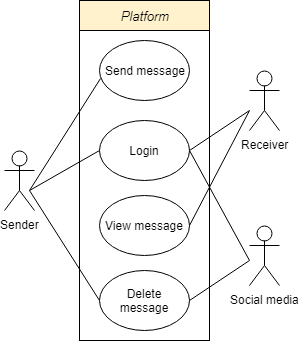
\includegraphics[width=0.75\linewidth]{Projectdoc/Assets/Illustrationer/simple-usecase-eng.png}
            \caption{Usecase diagram}
            \label{fig:usecase}
        \end{figure}
    \end{minipage}
    \begin{minipage}{.5\textwidth}
        \noindent
        Figure \ref{fig:usecase} on the left  describes a conceptual model of what the basic functionality of the inconspicuous communication platform looks like. The model describes how a sender, receiver and a external social media will interface with the system. The "Send message" action will be interfaced with by the sender and will deliver the message to the system for further processing. The "Login" action connects the sender, receiver and social media together. The "View message" action will be interfaced with by the receiver and displays a message from the system. The "Delete message" will be interfaced with by both the sender and the social media and will trigger a message deletion request to the system.
    \end{minipage}
\end{table}

\textbf{Use case \#1, Login.}\\
Object: The user should be prompted for a login, either through a personal social media, or though an anonymous bot.\\
Attributes: Selection of bot, Social media credentials.\\
Operations: Connect the user through the given credentials.\\
Manipulation: Set default settings through sub tap,  Set remember login credentials with checkbox.\\
Next Relationship: Send message[\#2], View message[\#3].\\\\
\newpage
\noindent
\textbf{Use case \#2, Send message.}\\
Object: The user has the option to select a category or thread to submit a new message.\\
Attributes: Selection of post relations, message content.\\
Operations: Post user generated message in relation to the selected thread or category.\\
Manipulation: None.\\
Next Relationship: Login[\#1], Send message[\#2], View message[\#3].\\\\
\noindent
\textbf{Use case \#3, View message.}\\
Object: The user has the option to select a specific message or thread to display.\\
Attributes: Category, Message, Thread.\\
Manipulation: Option to delete a message or thread (If user has ownership).\\
Next Relationship: Login[\#1], Send message[\#2], View message[\#3], Delete message[\#4].\\\\
\noindent
\textbf{Use case \#4, Delete message.}\\
Object: The user have the option to select a specefic message or thread to delete (if user contains ownership).\\
Attributes: Message, Thread, Ownership.\\
Manipulation: Delete a message or thread.\\
Next Relationship: Login[\#1], Send message[\#2], View message[\#3].\\

\end{document}